\chapter{Materials and methods}

\section{Computing resources}

Code development for this project was performed on a VANT MOOVE15 laptop with an 
Intel\regsup{} Core™ i5-1235U processor, 64 GB DDR4 RAM, and 2 TB NVMe SSD, 
running Ubuntu 24.04.1 LTS.

% Code for this project was developed on a VANT MOOVE15 laptop. This device is 
% equipped with an Intel\regsup{} Core™ i5-1235U processor, 64 GB of DDR4 RAM at 
% 3200 MHz, integrated Intel Xe Graphics, and a 2 TB NVMe SSD with a PCIe 4.0$\times$4 
% interface, all running on the Ubuntu 24.04.1 LTS operating system.

% For the development of the code and the fine-tuning of certain methods in this 
% project, a VANT MOOVE15 laptop was utilized. This laptop is equipped with an 
% Intel\regsup{} Core™ i5-1235U processor, 64 GB of DDR4 3200 MHz RAM, integrated Intel Xe 
% Graphics, and a 2 TB NVMe SSD with a PCIe 4.0$\times$4 interface, all running on the 
% Ubuntu 24.04.1 LTS operating system. 

Due to the computational demands of the tasks required to achieve the proposed
objectives, the CNIO High-Performance Computing (HPC) cluster was utilized. 
The cluster currently features 12 compute nodes with configurations as detailed 
in \textbf{Table \ref{tab:nodes}}.

\begingroup
\vspace{0.30cm}
\footnotesize

\begin{longtable}{>{\RaggedRight\arraybackslash}p{1.5cm} 
                  >{\RaggedRight\arraybackslash}p{2.5cm} 
                  >{\RaggedRight\arraybackslash}p{2cm}
                  >{\RaggedRight\arraybackslash}p{2cm}
                  >{\RaggedRight\arraybackslash}p{4cm}}
    \captionsetup{labelfont=bf, font=footnotesize}
    \caption[Technical specifications of computing nodes in CNIO's HPC cluster]
    {Technical specifications of computing nodes in CNIO's HPC cluster 
    \cite{noauthor_usage_nodate}.}\label{tab:nodes}\\
    
    \toprule
    \rowcolor{lightgray}
    \textbf{Count} & \textbf{Node names} & \textbf{CPU cores} & \textbf{RAM} & \textbf{GPUs} \\ 
    \midrule
    \endfirsthead
    
    \multicolumn{5}{@{}l}{\RaggedRight \textbf{\tablename\ \thetable{}} -- Continued} \\
    \\
    \toprule
    \rowcolor{lightgray}
    \textbf{Count} & \textbf{Node names} & \textbf{CPU cores} & \textbf{RAM} & \textbf{GPUs} \\ 
    \midrule
    \endhead
    \\
    \midrule 
    \multicolumn{5}{r}{\footnotesize Continued on next page} \\
    \endfoot
    
    \bottomrule
    \endlastfoot

    \\
    1     & bc001      & 24  & 32 GB  & -- \\
    \\
    6     & bc00[2-7]  & 52  & 512 GB & -- \\
    \\
    3     & bc00[8-10] & 128 & 1 TB   & -- \\
    \\
    1     & hm001      & 224 & 2 TB   & -- \\
    \\
    1     & gp001      & 112 & 768 GB & 3 x Nvidia A100 80 GB \\
    \\

\end{longtable}
\endgroup


    % \begin{itemize}[label=\tiny\raise.5ex\hbox{•}, leftmargin=\parindent]

    %     \item Two login nodes (40 cores, 392 GB RAM each)
        
    %     \item Nine compute nodes:
        
    %     \begin{itemize}

    %         \item Six nodes: 52 cores, 512 GB RAM each
            
    %         \item Three nodes: 64 cores, 768 GB RAM each
            
    %         \item One high-memory node: 224 cores, 2 TB RAM
            
    %     \end{itemize}

    %     \item One GPU node with three Nvidia A100 80 GB GPUs
        
    %     \item Storage: 54 TB RAID-10 for home directories and 512 TB Lustre 
    %     system for computation

    % \end{itemize}
    
The cluster's storage resources include 52 TB of standard storage space for 
user home directories, complemented by 512 TB of high-performance storage 
optimized for compute job input and output operations. From this 
high-performance storage, 30 TB was specifically allocated as project space 
for code execution and data generation.

% However, the volume and computational demands of the tasks required to achieve 
% the project's objectives far exceed the capabilities of any laptop or workstation. 
% Consequently, the High-Performance Computing (HPC) cluster at CNIO, hereafter 
% referred to as ``the cluster'', was used.

% The cluster currently comprises two login nodes operating in active/passive 
% mode, each with 40 cores and 392 GB of RAM. It includes a total of 728 compute 
% cores distributed across nine standard compute nodes: six nodes with 52 cores 
% and 512 GB of RAM each, three nodes with 64 cores and 768 GB of RAM each, and a 
% high-memory node with 224 cores and 2 TB of RAM. Additionally, there is a 
% dedicated GPU node equipped with three Nvidia A100 80 GB GPUs. Local storage 
% consists of 48 disks of 4 TB each in a dual-channel enclosure organized into a 
% RAID-10 unit, providing an effective available storage of 54 TB for users' home 
% directories, along with a high-performance Lustre storage system offering 512 TB 
% of effective available storage for computation (CNIO Bioinformatics Unit 
% Documentation, 2024). A project space of 60 TB of the cluster's high-performance 
% storage was dedicated to generate and store the data. 

\section{Software tools}

Visual Studio Code served as the primary interface for cluster access via SSH 
and code development. The implementation primarily utilized Bash, Python, and R 
programming languages.

The cluster operates under Slurm Workload Manager, a Linux/Unix-based system for 
HPC resource management. Workflow integration was accomplished through 
Snakemake, a Python-based workflow manager that enables isolated software 
environments for each workflow step using Conda, thus avoiding node-specific 
installations and potential compatibility issues.

Miniforge, a minimal Conda distribution preconfigured with conda-forge as the 
default software, was installed to manage Conda environments. The Bioconda 
software repository was added to access specialized bioinformatics packages.

A detailed compilation of all software tools utilized throughout this research
is presented in \textbf{Table~\ref{tab:software}}. The subsequent subsections 
detail how these tools were strategically integrated into comprehensive 
workflows to address the project's specific objectives.

% Visual Studio Code was used as the main interface to access the cluster via 
% Secure Shell (SSH) and write all the code used in this work. The main programming 
% languages employed were Bash, Python, and R.

% The cluster's resources and job scheduling are managed by Slurm Workload 
% Manager, a software system designed for Linux/Unix-based high-performance 
% computing environments. To integrate workflows into this tool, Snakemake, 
% a Python-based workflow management system, was employed. One of the key 
% advantages of Snakemake is its ability to define isolated software environments 
% for each rule in the workflow using Conda. This feature eliminates the need to 
% install programs on every cluster node that will utilize them, streamlining the 
% workflow process and reducing potential compatibility issues. 

% Miniforge, a minimalist distribution, was installed to facilitate the use of 
% Conda on the cluster. This distribution is preconfigured to use the conda-forge 
% channel as the default package source. Additionally, the Bioconda channel, which 
% specializes in bioinformatics software, was added to expand the range of 
% available packages.

% All the software tools used for this work, including those recently discussed, 
% are collected and detailed in \textbf{table~\ref{tab:software}}. Following 
% subsections will address how these tools have been used to generate workflows to 
% solve the specific objectives of this project.

% \begingroup
% \vspace{0.35cm}
% \footnotesize
% \begin{longtable}{>{\RaggedRight\arraybackslash}p{3.5cm} >{\RaggedRight\arraybackslash}p{4cm} >{\RaggedRight\arraybackslash}p{7.25cm}}
%     \captionsetup{labelfont=bf, font=footnotesize}
%     \caption[Software tools used in this work]{\RaggedRight \footnotesize Software tools used in this work.}
%     \label{tab:software}\\
    
%     \toprule
%     \rowcolor{lightgray}
%     \textbf{Name} & \textbf{Reference} & \textbf{Source} \\ 
%     \midrule
%     \endfirsthead
    
%     \multicolumn{3}{@{}l}{\RaggedRight \tablename\ \thetable{} -- Continued} \\
%     \\
%     \toprule
%     \rowcolor{lightgray}
%     \textbf{Name} & \textbf{Reference} & \textbf{Source} \\ 
%     \midrule \\
%     \endhead \\
%     \midrule 
%     \multicolumn{3}{r}{\footnotesize Continued on next page} \\
%     \endfoot
    
%     \bottomrule
%     \endlastfoot
    
%     \\
%     Visual Studio Code v1.93.1   & Microsoft, 2024              & \url{https://github.com/microsoft/vscode}          \\
%     \\
%     Snakemake v8.29.6            & Mölder et al., 2021          & \url{https://github.com/snakemake/snakemake}       \\
%     \\
%     Miniforge v24.7.1            & conda-forge community, 2024  & \url{https://github.com/conda-forge/miniforge}     \\
%     \\
%     VISOR v1.1.2.1               & Bolognini et al., 2020       & \url{https://github.com/davidebolo1993/VISOR}      \\
%     \\
%     minimap2 v2.28               & Li, 2018                     & \url{https://github.com/lh3/minimap2}              \\          
%     \\
%     SAMtools v1.21               & Danecek et al., 2021         & \url{https://github.com/samtools/samtools}         \\
%     \\
%     SAVANA v1.2.2                & Elrick et al., 2024          & \url{https://github.com/cortes-ciriano-lab/savana} \\
%     \\
%     Severus v1.2                 & Keskus et al., 2024          & \url{https://github.com/KolmogorovLab/Severus}     \\
%     \\
%     Sniffles2 v2.4               & Smolka et al., 2024          & \url{https://github.com/fritzsedlazeck/Sniffles}   \\
%     \\
%     SVision-Pro v2.0             & Wang et al., 2024            & \url{https://github.com/sonGBowang125/SVision-pro} \\
%     \\
%     BEDtools vX.X                & Anybody, XXXX                & \url{https://github.com/arq5x/bedtools2}           \\
%     \\
%     GW vX.X                      & Cleal K., 2024               & \url{https://github.com/kcleal/gw   }              \\
%     \\
%     UCSC Genome Browser v2024    & Anybody, 2024                & \url{https://genome.ucsc.edu/index.html}           \\
%     \\
%     draw.io v24.7.17             & ????                         & \url{https://github.com/jgraph/drawio-desktop}     \\
%     \\
%     Rstudio v2024.04.2           & ????                         & \url{https://github.com/rstudio/rstudio}           \\      
%     \\
%     dorado \\
%     \\
%     modkit \\
%     \\
%     Clair3 \\
%     \\
%     ClairS \\
%     \\

% \end{longtable}
% \endgroup

\subsection{Simulating long-read data and SV calling}

In the absence of curated long-read gold-standard datasets, testing SV calling methods 
with real biological datasets demands complex experimental procedures that are 
time-consuming, expensive, and potentially biased. In contrast, \textit{in silico} 
approaches provide an efficient and accurate alternative to evaluate SV caller 
performance, where the ground truth is known.

% The creation of new biological datasets with specific characteristics for SV 
% calling tests involves conducting complex biological experiments that demand a
% a significant investment of time and financial resources. Additionally, these 
% experiments may be subject to inherent biases that could compromise the quality 
% and representativeness of the obtained data. In contrast, \textit{in silico} 
% simulations enable an inexpensive and accurate estimation of precision and 
% recall of SV calling methods. 

\subsubsection{Data simulator}

VISOR toolkit was selected for haplotype-specific simulations of simple and 
complex SVs. Their VISOR LASeR module uses an error model trained on ONT R10.4.1 
reads from 2023, provided by Badread \cite{wick_badread_2019}.

% VISOR was selected as the tool for haplotype-specific simulations of 
% simple and complex SVs. This tool was chosen for its ability to generate long 
% reads with an error profile that closely matches those obtained through 
% sequencing with an ONT R10.4 flow cell.

\subsubsection{SV callers}

A set of SV calling tools was selected based on two key criteria: ONT 
long-read compatibility and somatic SV detection ability. Each selected caller 
provides distinct features valuable for this analysis:

% For this study, a set of SV callers was carefully selected based on specific 
% criteria: compatibility with ONT long reads and capability to detect somatic 
% SVs. In addition, each tool offers unique features that make them valuable for 
% this analysis:

\begin{itemize}[label=\tiny\raise.5ex\hbox{•}, leftmargin=\parindent]

    % \item \textbf{SAVANA}. Employs a machine learning model, trained on an 
    % extensive dataset of tumor-normal paired samples, to precisely identify 
    % somatic SVs and copy number aberrations (CNAs) in clinical  samples.
    
    % \item \textbf{Severus}. Designed for tumor/normal comparison analysis, 
    % supports multiple tumor samples, and uses a breakpoint graph framework to 
    % model complex chromosomal rearrangements.

    % \item \textbf{Sniffles2}. It was one of the first SV callers for ONT 
    % long reads, its first version appeared in 2018 and since then it continues 
    % to receive regular upgrades.

    % \item \textbf{SVision-pro}. Uses a genome-to-genome representation module 
    % encoding genomic features from two samples to an image, from which a 
    % neural-network recognition module comparatively recognizes SVs.

    \item \textbf{SAVANA}: Implements a machine learning model trained on 
    tumor-normal paired samples to detect somatic SVs and copy number 
    aberrations (CNAs) in clinical cases.

    \item \textbf{Severus}: Specializes in tumor/normal comparative analysis, 
    supporting multi-tumor samples and employing breakpoint graph frameworks 
    for complex chromosomal rearrangement detection.

    \item \textbf{Sniffles2}: A pioneering ONT long-read SV caller since 2018, 
    maintaining continuous development and regular updates.

    \item \textbf{SVision-pro}: Employs a neural network-based approach that 
    converts genomic features from paired samples into image representations 
    for comparative SV detection.
    
\end{itemize}

\subsubsection{Generation and calling of SVs}

A comprehensive workflow for VISOR-based simulations and SV calling analysis was 
developed. The complete code and documentation are available in the following
repository: \url{https://github.com/villena-francis/visor-simulations}. 
\textbf{Figure \ref{fig:visor-sim}} illustrates the key workflow steps.

% A comprehensive workflow was established to generate simulations using VISOR 
% and run them for SV call analysis. The associated code and usage instructions 
% are accessible in the following repository: 
% \url{https://github.com/villena-francis/visor-simulations}. 
% \textbf{Figure \ref{fig:visor-sim}} presents a simplified overview of the key 
% steps involved in this process.

\newpage

\begin{figure}[H]
    \centering
    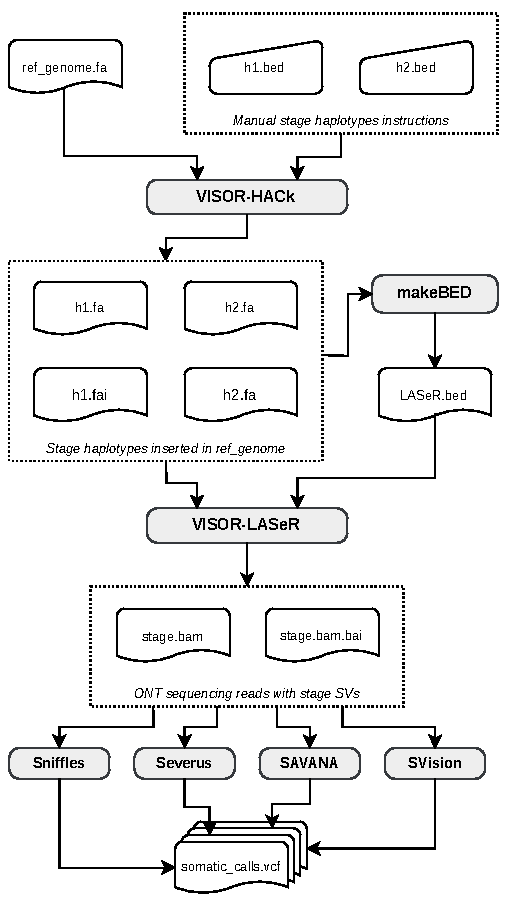
\includegraphics[scale=1.3]{img/visor-simulations.pdf}
    \caption[Simplified version of ``visor-simulations'' workflow for long-read 
    simulation and SV calling]{Simplified version of ``visor-simulations'' 
    workflow for long-read simulation and SV calling. VISOR-HACk generates FASTA 
    files (reference sequences) with incorporated SVs using a reference genome and 
    BED-formatted haplotype instructions (tab-delimited genomic coordinates). 
    The makeBED script creates a BED file (genomic intervals) from maximum 
    chromosome sizes extracted from haplotype FASTAs. VISOR-LASeR then generates 
    BAM files (aligned sequencing reads) and their indexes (.bai) using these 
    files as input. each generating its corresponding variant call file (VCF) 
    containing the identified SVs. The workflow parallelizes simulations 
    across stages using configuration files and wildcards, producing 
    multiple replicates at various sequencing coverages with corresponding 
    normal samples.}
    % \caption[Simplified version of ``visor-simulations'', a workflow for 
    % simulating long-read data and testing SV callers]{Simplified version of 
    % ``visor-simulations'', a workflow for simulating long-read data and testing 
    % SV callers. Using a reference genome and BED format instructions for the 
    % stage haplotypes (a set of genetic variations found in one of the pairs of 
    % each chromosome), VISOR-HACk generates FASTA files with the structural 
    % variants (SVs) incorporated. The makeBED script extracts the maximum 
    % chromosome sizes from the haplotype FASTA files to create a BED file. This 
    % file, along with the haplotype FASTA files, serves as input for VISOR-LASeR 
    % to generate BAM long-reads and their respective indexes (.bai). As a final 
    % step, somatic variant calls for the BAM long-read are performed using SAVANA, 
    % Severus, Sniffles2 and SVision-Pro. Actual workflow parallelizes the 
    % generation of simulations for each stage using a configuration file and a 
    % set of wildcards. It produces multiple replicates at different sequencing 
    % coverages and generates a normal sample for each coverage to facilitate 
    % somatic variant calling. Diagram generated with draw.io.}
    \label{fig:visor-sim}
\end{figure}

\subsubsection{Simulation stages}

Each stage incorporates specific SVs into the GRCh38 reference genome, simulated 
at four coverage levels: 30x, 50x, 100x, and 200x. The initial stage generated 
one normal sample and three tumor replicates per coverage level, totaling 16 BAM 
simulations. Subsequent stages reused the normal samples, requiring only 12 
simulations each through the automation provided by the ``visor-simulations'' 
workflow. 

The stage generated for this project (v1) incorporated six chromosomal 
aberrations characteristic of multiple myeloma, including tandem duplications, 
deletions, and various types of translocations (\textbf{Table~\ref{tab:stagesV1}}). 
Breakpoint coordinates for these structural variants were approximately 
determined using the UCSC Genome Browser, as specific locations were not 
detailed in the clinical literature.

% A stage incorporates specific SVs into the GRCh38 reference genome, simulated 
% at four coverage levels: 30x, 50x, 100x, and 200x. The initial stage generated 
% one normal sample and three tumor replicates per coverage level, totaling 16 BAM 
% simulations. Subsequent stages reused the normal samples, requiring only 12 
% simulations each gracias a la automatización de “visor-simulations” workflow.

% The first stage (v1) incorporated three characteristic multiple myeloma 
% chromosomal aberrations plus three additional SVs to test diverse variant 
% types (\textbf{Table~\ref{tab:stagesV1}}). Breakpoint coordinates were 
% determined using the UCSC Genome Browser [citar], as precise locations were not 
% specified in the literature.

% Each stage consists of a set of SVs to be inserted into 
% the GRCh38 reference genome for read simulation at four levels of average 
% coverage: 30x, 50x, 100x, and 200x. For the first stage, a ``normal'' sample and 
% three ``tumour'' replicates were generated for each coverage level, resulting in 
% a total of 16 simulations of long-read BAM files. In subsequent stages, the 
% normal samples were reused, leading to 12 simulations per stage.

% First stage (v1) of simulations was based on a set of three characteristic 
% chromosomal aberrations associated with multiple myeloma, along with three 
% additional, more speculative to account for other types of SVs
% (\textbf{Table~\ref{tab:stagesV1}}). The exact breakpoints were not specified in 
% the scientific literature, so they were inferred based on the location of the 
% affected region and their respective coordinates in the GRCh38 reference genome 
% using the UCSC Genome Browser [citar].

\begingroup
\vspace{0.35cm}

\footnotesize

\begin{longtable}{>{\RaggedRight\arraybackslash}p{2.5cm} 
                  >{\RaggedRight\arraybackslash}p{10.5cm} 
                  >{\RaggedLeft\arraybackslash}p{1.75cm}}
    \captionsetup{labelfont=bf, font=footnotesize}
    \caption[Simulated chromosomal aberrations characteristic of Multiple 
    Myeloma]{\footnotesize Simulated chromosomal aberrations characteristic of 
    Multiple Myeloma \cite{aksenova_genome_2021}. Size values represent the final 
    length in base pairs (bp) after genome insertion. Tandem duplication 
    consists of a 2,030,586 bp fragment repeated four times. Input files for 
    VISOR read simulation available at 
    \url{https://github.com/villena-francis/visor-simulations/tree/main/resources/v1}}. 
    \label{tab:stagesV1}\\
    
    \toprule
    \rowcolor{lightgray}
    \textbf{SV type} & \textbf{Description} & \textbf{Size (pb)} \\ 
    \midrule
    \endfirsthead
    
    \multicolumn{3}{@{}l}{\RaggedRight \textbf{\tablename\ \thetable{}} -- Continued} \\
    \\
    \toprule
    \rowcolor{lightgray}
    \textbf{SV type} & \textbf{Description} & \textbf{Size (pb)} \\ 
    \midrule
    \\
    \endhead
    \\
    \midrule 
    \multicolumn{3}{r}{\footnotesize Continued on next page} \\
    \endfoot
    
    \bottomrule
    \endlastfoot

    \\
    Tandem \mbox{duplication}         & Amplification of chromosome 1q (1q21+), representing one of the most frequent structural cytogenetic abnormalities in Multiple Myeloma, occurring in approximately 40\% of cases .     & 10152930 \\
    \\
    Deletion                          & Deletion of chromosome 17p, present in approximately 10\% of Multiple Myeloma cases, serves as a significant poor prognostic indicator. The minimally deleted region at locus 17p13 encompasses the tumor suppressor gene TP53 & 234564 \\
    \\
    Translocation \mbox{(reciprocal)} & Chromosomal rearrangement involving the immunoglobulin heavy chain (IGH) gene at 14q32, a hallmark genetic event in Multiple Myeloma pathogenesis.                                                  & 1502367  \\
    \\
    Translocation \mbox{(cut-paste)}  & Rearrangement involving CDKN2A, a crucial tumor suppressor gene whose inactivation through mutations or deletions is among the most frequent alterations in human cancers, second only to TP53 alterations. & 31271 \\
    \\
    Translocation \mbox{(copy-paste)} & Structural variation affecting the KRAS oncogene region, whose alterations are frequently associated with Multiple Myeloma progression.  & 45683 \\
    \\
    Inversion                         & Chromosomal inversion at 6q25.1, included as a control variant to validate the detection capabilities of structural variant analysis pipelines, although not typically characteristic in Multiple Myeloma.          & 3600001  \\
    \\

\end{longtable}
\endgroup

% (Hanamura, 2021)

% Second (v2) and third (v3) stages were implemented to comprehensively analyze 
% the impact of SV sizes on detection and characterization. These stages utilized 
% the same SV types and initial breakpoints as the first stage but adjusted the 
% affected region lengths. Stage v2 employed 1,000 bp regions, while v3 used 
% 100,000 bp regions. This approach allows a more comprehensive examination of how 
% different SV sizes influence the accuracy of detection methods.

\newpage 

\subsection{Benchmarking of SV callers}

\subsubsection{Data subsampling for local device processing}

Visual inspection of BAM file reads is essential for validating simulation 
quality and SV caller accuracy. Due to cluster limitations with graphical 
interfaces, this analysis requires local processing. We developed a workflow to 
split whole-genome BAM files by chromosome, available at 
\url{https://github.com/villena-francis/bam-splitter}. 
\textbf{Figure \ref{fig:bam-splitter}} illustrates the workflow's key 
components.

% Confirming the accuracy and identifying errors of SV callers requires a 
% preliminary assessment of simulation quality through visualization of BAM file 
% reads. Since the cluster cannot execute graphical interfaces, this task must be 
% performed on a local machine. To streamline this process, a workflow was 
% developed for chromosomal splitting of whole-genome BAM files. The code and 
% usage instructions are accessible in the following repository: 
% \url{https://github.com/villena-francis/bam-splitter}.
% An overview of the key steps involved in this process is presented in 
% \textbf{figure \ref{fig:bam-splitter}}.

\begin{figure}[H]
    \centering
    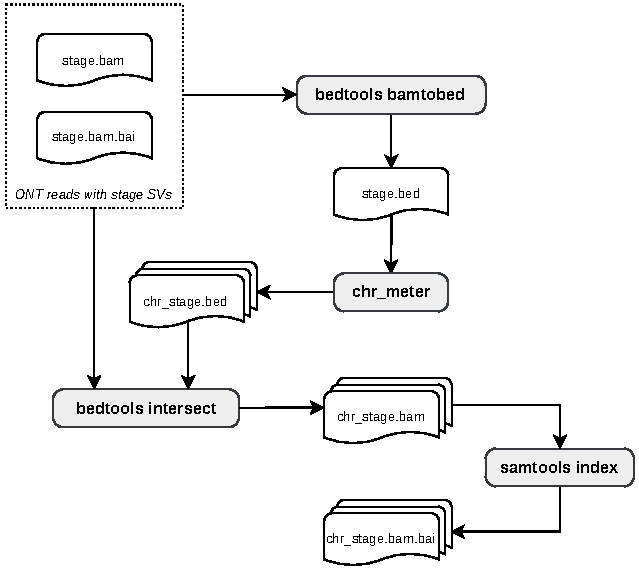
\includegraphics[scale=1.3]{img/bam-splitter.pdf}
    \caption[Simplified version of ``bam-splitter'' workflow for chromosomal 
    splitting of BAM files]{Simplified version of ``bam-splitter'' workflow for 
    chromosomal splitting of BAM files. The process begins with bedtools 
    bamtobed generating a comprehensive BED file of chromosome coordinates. 
    The chr\_meter script then creates individual BED files for selected 
    chromosomes, which bedtools intersect uses to produce chromosome-specific 
    BAM files. Samtools generates corresponding indexes for each BAM file. The 
    workflow employs configuration files and wildcards to parallelize chromosome 
    processing.}
    % \caption[Simplified version of ``bam-splitter'', a workflow for chromosomal 
    % splitting of whole-genome BAM files.]{Simplified version of ``bam-splitter'', 
    % a workflow for chromosomal splitting of whole-genome BAM files. First, the 
    % bedtools bamtobed function is used to generate a BED file containing the 
    % start and end coordinates of all chromosomes. Subsequently, for the 
    % specifically selected chromosomes, the chr\_meter script is employed to 
    % create independent BED files for each of them. These individual BED files 
    % are crucial for the next step, in which the bedtools intersect function uses 
    % them to produce separate copies in BAM format of the chosen chromosomes. 
    % Finally, samtools utilizes these individual BAM files to generate their 
    % corresponding indexes. Actual workflow parallelizes the separate copies for 
    % each chromosome using a configuration file and a set of wildcards. Diagram 
    % generated with draw.io.}
    \label{fig:bam-splitter}
\end{figure}

\subsubsection{Visualization of long read alignments}

Chromosomal BED visualization was conducted using Genome-Wide (GW), an advanced, 
ultra-fast genome browser capable of exploring extensive genomic regions and 
complete chromosomes. GW's specialized features, particularly its VCF-based 
manual curation capability, facilitated rapid validation of SV caller 
predictions.

% Inspection of chromosomal BEDs was performed through Genome-Wide (GW), a novel 
% ultra-fast and interactive genome browser that enables the exploration of 
% extensive genomic regions and entire chromosomes. GW incorporates specialized 
% features, including manual curation facilitated by information extracted from 
% input VCF files. This functionality was exploited to quickly review the hits 
% detected by the SV callers.

\subsubsection{Classification of SV calling results}

Performance evaluation of SV callers employed a binary classification framework 
with the following criteria:

\begin{itemize}[label=\tiny\raise.5ex\hbox{•}, leftmargin=\parindent]

    \item \textbf{True Positives (TP)}: Successfully detected simulated SVs.
    
    \item \textbf{False Positives (FP)}: Caller-identified SVs absent in 
    simulation, verified through read inspection.
    
    \item \textbf{False Negatives (FN)}: Simulated SVs present in reads but 
    undetected by caller.

\end{itemize}

True Negatives (TN) were excluded from this analysis due to their 
inapplicability in SV calling evaluation, given the vast genomic space and 
nature of SV detection methods.

% To evaluate the performance of SV callers, we employed a binary classification 
% framework. The evaluation criteria were as follows:

% \begin{itemize}[label=\tiny\raise.5ex\hbox{•}, leftmargin=\parindent]

%     \item \textbf{True Positives (TP)}: simulated SVs successfully detected by 
%     the caller.

%     \item \textbf{False Positives (FP)}: SVs identified by the caller but not 
%     present in the simulation, confirmed absent through read verification.

%     \item \textbf{False Negatives (FN)}: simulated SVs confirmed present through 
%     read verification but undetected by the caller.

% \end{itemize}

% It is crucial to emphasize that True Negatives (TN) could not be quantified and 
% are not applicable in the conventional sense for SV calling evaluations. This 
% limitation arises from the inherent nature of SV detection methodologies and the 
% vast genomic landscape in which SVs can occur.

\subsubsection{Metrics used}

Due to the impossibility of quantifying true negatives in SV calling, we 
employed TN-independent metrics:

\begin{enumerate}[leftmargin=\parindent]
    
    \item \textbf{Recall}: Proportion of correctly identified positive cases
    \begin{equation}
        \label{eq:recall}
        Recall = \frac{TP}{TP + FN}
    \end{equation}

    \item \textbf{Precision}: Accuracy of positive predictions
    \begin{equation}
        \label{eq:precision}
        Precision = \frac{TP}{TP + FP}
    \end{equation}

    \item \textbf{F1 Score}: Harmonic mean of precision and recall
    \begin{equation}
        \label{eq:f1score}
        F1 = 2 \cdot \frac{precision \cdot recall}{precision + recall}
    \end{equation}

\end{enumerate}

Computational efficiency was evaluated using Slurm-generated statistics: CPU/GPU 
utilization (cores), RAM consumption (GB), and execution time (minutes).

\subsubsection{Data Visualization and Statistical Analysis}

Metric analysis and visualization were implemented through R scripts available 
at \url{https://github.com/villena-francis/master_thesis/tree/main/data/cluster_bmk}.

% Given the inability to quantify true negatives (TN) in this context, we focused 
% on metrics that do not require these values to assess SV calling performance:

% \begin{enumerate}[leftmargin=\parindent]

%     \item \textbf{True Positive Rate (TPR)} or \textbf{Recall}: proportion 
%     of actual positive cases correctly identified.
%     \begin{equation}
%         \label{eq:recall}
%         Recall = \frac{TP}{TP + FN}
%     \end{equation}

%     \item \textbf{Precision}: accuracy of positive predictions.
%     \begin{equation}
%         \label{eq:precision}
%         Precision = \frac{TP}{TP + FP}
%     \end{equation}

%     \item \textbf{F1 Score}: harmonic mean of precision and sensitivity, 
%     providing a balanced assessment of overall performance.
%     \begin{equation}
%         \label{eq:f1score}
%         F1 = 2 \cdot \frac{precision \cdot recall}{precision + recall}
%     \end{equation}

% \end{enumerate}

% Additionally, we utilized the statistics generated by Slurm for each job to 
% assess the computational efficiency of VISOR simulations and SV callers. These 
% metrics included CPU/GPU load (cores), RAM usage (GB), and execution time 
% (minutes). 

% Computation and visualization of these metrics were performed using a custom R 
% script, available at \url{https://github.com/villena-francis/a-repo-for-that}.


% Generación de facet grid usando R para el rendimiento computacional y exitos
% de las herramientas https://r-charts.com/ggplot2/facets/







